\subsection{Evolutionary Policy Search}

First, we ran evolutionary policy search on the Toy Problem discussed in Section 4.4 with an MLP Policy with 4 hidden units. We used the evolutionary parameters as detailed in Section 4.2. Figure \ref{Fitness during Evolutionary Algorithm} shows the fitness of the best policy in the pool over the number of epochs. This was averaged over ten runs and 95\% confidence intervals are shown. 

\begin{figure}[ht]
  \centering
  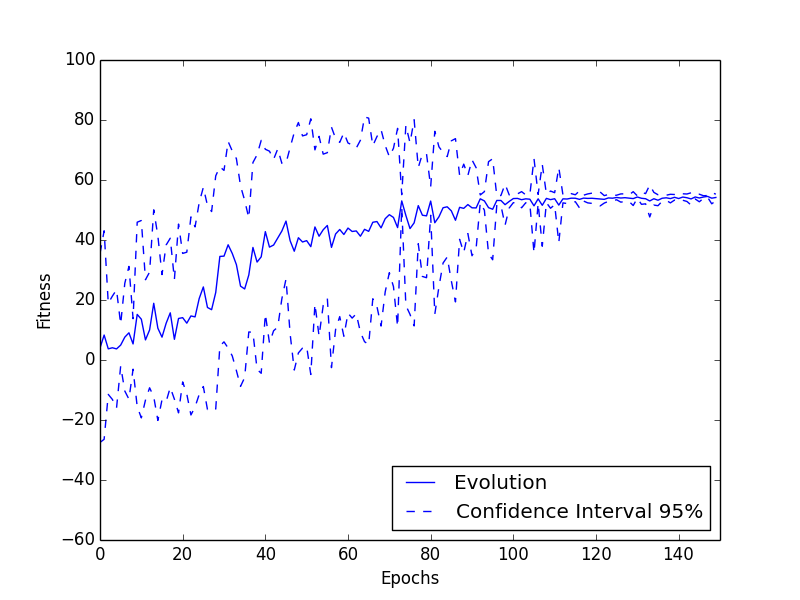
\includegraphics[scale=0.5]{images/evo.png}
  \caption{Fitness during Evolutionary Algorithm}\label{Fitness during Evolutionary Algorithm}
\end{figure}

Figure \ref{Example policy learned with evolutionary algorithm} shows the performance of an example policy found with the evolutionary policy search algorithm, after 200 epochs. The wind is sampled from a uniform distribution between 0 and 0.5. Note that for all wind strengths, this policy reaches the goal. 

\begin{figure}[ht]
  \centering
  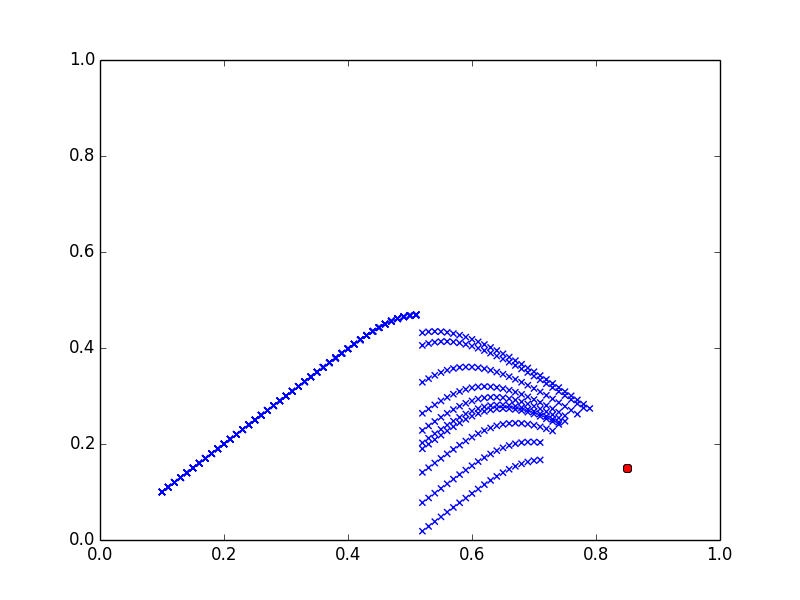
\includegraphics[scale=0.5]{images/evo_result.png}
  \caption{Example policy learned with evolutionary algorithm}\label{Example policy learned with evolutionary algorithm}
\end{figure}

\subsection{Co-Evolutionary Policy Search}

The results for Co-Evolutionary Policy Search are shown in Figure \ref{Fitness during Co-Evolutionary Algorithm}.  

\begin{figure}[ht]
  \centering
  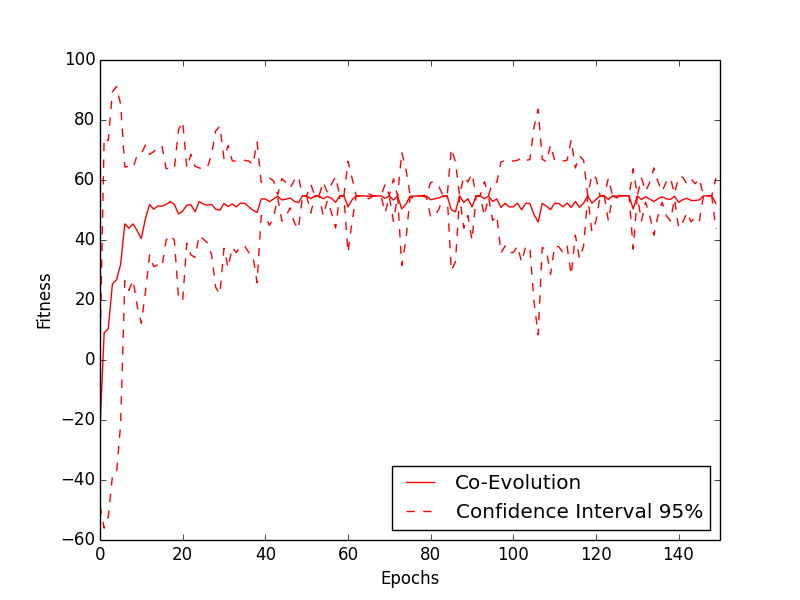
\includegraphics[scale=0.5]{images/co_evo.png}
  \caption{Fitness during Co-Evolutionary Algorithm}\label{Fitness during Co-Evolutionary Algorithm}
\end{figure}

Once again, an MLP with 4 hidden units was trained, and the same general evolutionary parameters from Section 4.2 were used. An example policy trained with Co-Evolutionary Policy Search for 200 epochs is visualized in Figure \ref{Example policy learned with Co-Evolutionary algorithm}. This policy too is able to reach the goal for any wind strength.


\begin{figure}[ht]
  \centering
  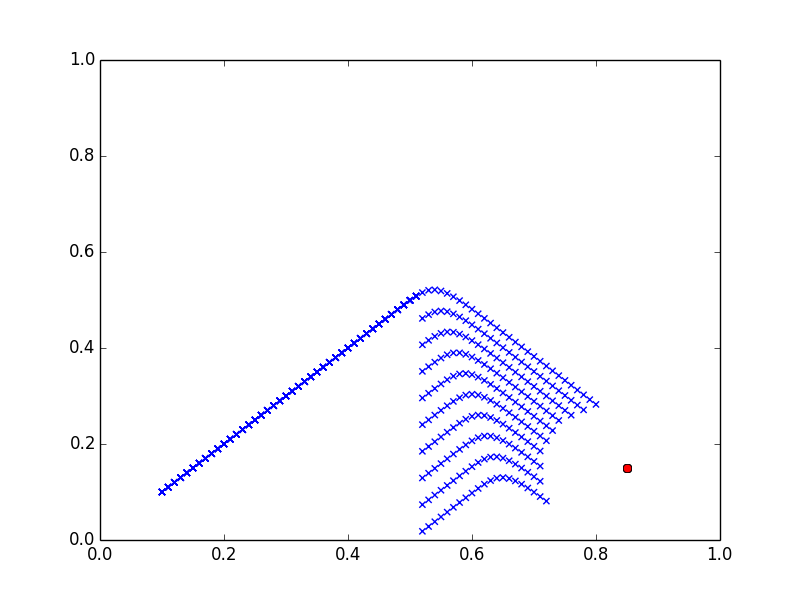
\includegraphics[scale=0.5]{images/co_evo_result.png}
  \caption{Example policy learned with Co-Evolutionary algorithm}\label{Example policy learned with Co-Evolutionary algorithm}
\end{figure}

\subsection{GP CEPS}

\subsection{Comparison}

